\documentclass[12pt,(landscape,a4paper),(portrait,a4paper)]{article}
\usepackage{lmodern}
\usepackage{amssymb,amsmath}
\usepackage{ifxetex,ifluatex}
\usepackage{fixltx2e} % provides \textsubscript
\ifnum 0\ifxetex 1\fi\ifluatex 1\fi=0 % if pdftex
  \usepackage[T1]{fontenc}
  \usepackage[utf8]{inputenc}
\else % if luatex or xelatex
  \ifxetex
    \usepackage{mathspec}
  \else
    \usepackage{fontspec}
  \fi
  \defaultfontfeatures{Ligatures=TeX,Scale=MatchLowercase}
\fi
% use upquote if available, for straight quotes in verbatim environments
\IfFileExists{upquote.sty}{\usepackage{upquote}}{}
% use microtype if available
\IfFileExists{microtype.sty}{%
\usepackage{microtype}
\UseMicrotypeSet[protrusion]{basicmath} % disable protrusion for tt fonts
}{}
\usepackage[margin=1in]{geometry}
\usepackage{hyperref}
\hypersetup{unicode=true,
            pdftitle={计量经济学Eviews实验指导书},
            pdfauthor={胡华平},
            pdfborder={0 0 0},
            breaklinks=true}
\urlstyle{same}  % don't use monospace font for urls
\usepackage{longtable,booktabs}
\usepackage{graphicx,grffile}
\makeatletter
\def\maxwidth{\ifdim\Gin@nat@width>\linewidth\linewidth\else\Gin@nat@width\fi}
\def\maxheight{\ifdim\Gin@nat@height>\textheight\textheight\else\Gin@nat@height\fi}
\makeatother
% Scale images if necessary, so that they will not overflow the page
% margins by default, and it is still possible to overwrite the defaults
% using explicit options in \includegraphics[width, height, ...]{}
\setkeys{Gin}{width=\maxwidth,height=\maxheight,keepaspectratio}
\IfFileExists{parskip.sty}{%
\usepackage{parskip}
}{% else
\setlength{\parindent}{0pt}
\setlength{\parskip}{6pt plus 2pt minus 1pt}
}
\setlength{\emergencystretch}{3em}  % prevent overfull lines
\providecommand{\tightlist}{%
  \setlength{\itemsep}{0pt}\setlength{\parskip}{0pt}}
\setcounter{secnumdepth}{5}
% Redefines (sub)paragraphs to behave more like sections
\ifx\paragraph\undefined\else
\let\oldparagraph\paragraph
\renewcommand{\paragraph}[1]{\oldparagraph{#1}\mbox{}}
\fi
\ifx\subparagraph\undefined\else
\let\oldsubparagraph\subparagraph
\renewcommand{\subparagraph}[1]{\oldsubparagraph{#1}\mbox{}}
\fi

%%% Use protect on footnotes to avoid problems with footnotes in titles
\let\rmarkdownfootnote\footnote%
\def\footnote{\protect\rmarkdownfootnote}

%%% Change title format to be more compact
\usepackage{titling}

% Create subtitle command for use in maketitle
\newcommand{\subtitle}[1]{
  \posttitle{
    \begin{center}\large#1\end{center}
    }
}

\setlength{\droptitle}{-2em}
  \title{计量经济学Eviews实验指导书}
  \pretitle{\vspace{\droptitle}\centering\huge}
  \posttitle{\par}
\subtitle{Lab 4 多元线性回归及矩阵运算}
  \author{胡华平}
  \preauthor{\centering\large\emph}
  \postauthor{\par}
  \predate{\centering\large\emph}
  \postdate{\par}
  \date{2018/3/27}

\usepackage{xeCJK}
\setCJKmainfont{楷体}  % 字体可以更换
\setmainfont{Georgia} % 設定英文字型
\setromanfont{Georgia} % 字型
\setmonofont{Courier New}

%设置版式 垂直或水平
% You know, for landscape
\usepackage{lscape}
\usepackage{pdfpages}


% Make new page before each section
\let\stdsection\section
\renewcommand\section{\newpage\stdsection}

% pandoc does not parse latex env - https://groups.google.com/forum/?fromgroups=#!topic/pandoc-discuss/oZETB5Ii1Cw
\newcommand{\blandscape}{\begin{landscape}}
\newcommand{\elandscape}{\end{landscape}}

\begin{document}
\maketitle

\renewcommand{\figurename}{图}
\renewcommand{\contentsname}{目录}
\renewcommand{\tablename}{表}


%% maxwidth is the original width if it's less than linewidth
%% otherwise use linewidth (to make sure the graphics do not exceed the margin)
\makeatletter
\def\maxwidth{ %
  \ifdim\Gin@nat@width>\linewidth
    \linewidth
  \else
    \Gin@nat@width
  \fi
}
\makeatother

{
\setcounter{tocdepth}{3}
\tableofcontents
}
\newpage

\section{实验目的及要求}

\begin{itemize}
\tightlist
\item
  \textbf{目的}:掌握多元线性回归模型的估计、检验。
\item
  \textbf{要求}:在老师指导下完成多元线性回归模型的建立、估计、统计检验,得到正确的分析结果;能运用矩阵方法实现前述操作。
\end{itemize}

\section{实验原理}

\begin{itemize}
\tightlist
\item
  当多元线性回归模型在满足线性模型古典假设的前提下,最小二乘估计结果具有无偏性、有效性等性质,在此基础上进一步对估计所得的模型进行经济意义检验及统计检验。
\end{itemize}

\hypertarget{k}{%
\subsection{k变量线性回归模型的矩阵表达}\label{k}}

k变量总体回归模型(PRF)的代数表达式如下:

\begin{equation}
Y_i=\beta_1+\beta_2X_{2i}+\beta_2X_{2i}+\cdots++\beta_kX_{ki}+u_i
\label{eq:PRM-algebra} 
\end{equation}

如果样本数为n,则k变量总体回归模型矩阵表达为:

\begin{equation}
  \begin{bmatrix}
  Y_1 \\  Y_2 \\  \cdots \\  Y_n \\
  \end{bmatrix}  =
  \begin{bmatrix}
  1 &  X_{21} & X_{31} & \cdots &  X_{k1} \\
  1 &  X_{22} & X_{32} & \cdots &  X_{k2} \\
  \cdots &  \cdots & \cdots & \cdots &  \cdots \\
  1 &  X_{2n} & X_{3n} & \cdots &  X_{kn}
  \end{bmatrix}
  \begin{bmatrix}
  \beta_1 \\  \beta_2 \\  \vdots \\  \beta_k \\
  \end{bmatrix}+
  \begin{bmatrix}
  u_1 \\  u_2 \\  \vdots \\  u_n \\
  \end{bmatrix}
\label{eq:PRM-agbmat} 
\end{equation}

\begin{equation}
\mathbf{y} = \mathbf{X}\mathbf{\beta}+\mathbf{u}
\label{eq:PRM-matrix} 
\end{equation}

\begin{equation}
(n \times 1) = (n \times n) (k \times 1)+(n \times 1)
\end{equation}

\subsection{经典线性回归模型假定的矩阵表述}

\hypertarget{olsblue}{%
\subsection{OLS估计及BLUE性质证明的矩阵表达}\label{olsblue}}

\subsection{对回归系数进行显著性检验}

\subsection{对回归模型进行总体显著性检验}

\hypertarget{anova}{%
\subsubsection{方差分析表(ANOVA)的矩阵表述}\label{anova}}

\hypertarget{f}{%
\subsubsection{总体模型显著性的F检验}\label{f}}

\subsection{用多元回归做预测:矩阵表述}

\newpage

\section{实验内容}

\subsection{实验方案设计}

在Eviews中运用\textbf{矩阵方法},计算如下步骤:

\begin{itemize}
\tightlist
\item
  计算直线回归方程的回归系数向量(\(\mathbf{\hat{\beta}}\)),并写出样本回归模型(\(SRM\))。
\item
  计算回归误差方差(\(\hat{\sigma}^2\))和回归误差标准差(\(\hat{\sigma}\))。
\item
  计算回归系数的样本方差协方差矩阵(\(\widehat{var}\_\widehat{cov}\))。
\item
  得出回归系数的样本标准差向量(\(S_{\hat{\beta}}\))。
\item
  进行平方和分解,计算\(TSS\)、\(ESS\)和\(RSS\)。
\item
  计算判定系数\(R^2\),调整判定系数(\(\hat{R}^2\))。
\item
  计算样本t统计量(\(\mathbf{t^{\ast}_{\beta}}\)),并进行t假设检验。
\item
  对回归方程的进行样本外均值预测\(E(Y|X=X_0)\)
\item
  对回归方程的进行样本外个值预测\((Y_0|X=X_0)\)
\end{itemize}

\newpage

\subsection{实验背景------玫瑰的需求}

\textbf{玫瑰的需求}:表\ref{tab:rose-demand}给出美国底特律市区对玫瑰的季度需求数据。

\begin{verbatim}
## Warning in 1:dim(table_lab[1]): numerical expression has 2 elements: only
## the first used
\end{verbatim}

\begin{table}

\caption{\label{tab:rose-demand}玫瑰的需求(n=16)}
\centering
\begin{tabular}[t]{r|r|r|r|r|r}
\hline
YEAR & Q & X2 & X3 & X4 & X5\\
\hline
1971.3 & 11484 & 2.26 & 3.49 & 158.11 & 1\\
\hline
1971.4 & 9348 & 2.54 & 2.85 & 173.36 & 2\\
\hline
1972.1 & 8429 & 3.07 & 4.06 & 165.26 & 3\\
\hline
1972.2 & 10079 & 2.91 & 3.64 & 172.92 & 4\\
\hline
1972.3 & 9240 & 2.73 & 3.21 & 178.46 & 5\\
\hline
1972.4 & 8862 & 2.77 & 3.66 & 198.62 & 6\\
\hline
1973.1 & 6216 & 3.59 & 3.76 & 186.28 & 7\\
\hline
1973.2 & 8253 & 3.23 & 3.49 & 188.98 & 8\\
\hline
1973.3 & 8038 & 2.60 & 3.13 & 180.49 & 9\\
\hline
1973.4 & 7476 & 2.89 & 3.20 & 183.33 & 10\\
\hline
1974.1 & 5911 & 3.77 & 3.65 & 181.87 & 11\\
\hline
1974.2 & 7950 & 3.64 & 3.60 & 185.00 & 12\\
\hline
1974.3 & 6134 & 2.82 & 2.94 & 184.00 & 13\\
\hline
1974.4 & 5868 & 2.96 & 3.12 & 188.20 & 14\\
\hline
1975.1 & 3160 & 4.24 & 3.58 & 175.67 & 15\\
\hline
1975.2 & 5872 & 3.69 & 3.53 & 188.00 & 16\\
\hline
\end{tabular}
\end{table}

变量说明见表\ref{tab:label-show}:

\begin{table}

\caption{\label{tab:label-show}变量定义及说明}
\centering
\begin{tabular}[t]{l|l}
\hline
variable & label\\
\hline
YEAR & 年份.季度\\
\hline
Q & 玫瑰销售量(打)\\
\hline
X2 & 玫瑰批发价格(\$/打)\\
\hline
X3 & 石竹的平均批发价格(\$/打)\\
\hline
X4 & 家庭可支配收入(\$/周)\\
\hline
X5 & 时间趋势\\
\hline
\end{tabular}
\end{table}

~

请考虑如下两个需求函数:

\begin{equation}
Y_t=\hat{\alpha}_1+\hat{\alpha}_2X_{2t}+\hat{\alpha}_3X_{3t}+
\hat{\alpha}_4X_{4t}+\hat{\alpha}_5X_{5t}+e_{1t}
\label{eq:model1}
\end{equation}

\begin{equation}
ln(Y_t)=\hat{\beta}_1+\hat{\beta}_2ln(X_{2t})+\hat{\beta}_3ln(X_{3t})+\hat{\beta}_4ln(X_{4t})+\hat{\beta}_5X_{5t}+e_{2t}
\label{eq:model2}
\end{equation}

定制化的公式效果函数:

调用效果函数:

\begin{equation*}
ln(Y_t)=\hat{\beta}_1+\hat{\beta}_2ln(X_{2t})+\hat{\beta}_3ln(X_{3t})\hat{\beta}_4ln(X_{4t})+\hat{\beta}_5X_{5t}+e_{2t}
\label{eq:mathtext1}
\end{equation*}

调用chunk模型\eqref{eq:mmm} \begin{equation}
ln(Y_t)=\hat{\beta}_1+\hat{\beta}_2ln(X_{2t})+\hat{\beta}_3ln(X_{3t})\hat{\beta}_4ln(X_{4t})+\hat{\beta}_5X_{5t}+e_{2t}
\label{eq:mmm}
\end{equation}

chunk调用结果如下: \begin{equation}
ln(Y_t)=\hat{\beta}_1+\hat{\beta}_2ln(X_{2t})+\hat{\beta}_3ln(X_{3t})\hat{\beta}_4ln(X_{4t})+\hat{\beta}_5X_{5t}+e_{2t}
\label{eq:mmm}
\end{equation}

转换函数如下

请回答如下问题:

\begin{enumerate}
\def\labelenumi{\alph{enumi}.}
\item
  关于线性模型\eqref{eq:mmm},运用菜单操作,得到回归分析报告。\\
\item
  关于线性模型\eqref{eq:model1},在Eviews中运用矩阵方法,计算如下步骤:

  \begin{enumerate}
  \def\labelenumii{\arabic{enumii}.}
  \tightlist
  \item
    计算直线回归方程的回归系数向量(\(\mathbf{\hat{\beta}}\)),并写出样本回归模型(\(SRM_2\))。\\
  \item
    计算回归误差方差(\(\hat{\sigma}^2\))和回归误差标准差(\(\hat{\sigma}\))。\\
  \item
    计算回归系数的样本方差协方差矩阵(\(\widehat{var}\_\widehat{cov}(\mathbf{\hat{\beta}})\))。\\
  \item
    得出回归系数的样本标准差向量(\(\mathbf{S_{\hat{\beta}}}\))。\\
  \item
    进行平方和分解,计算\(TSS\)、\(ESS\)和\(RSS\)。\\
  \item
    计算判定系数\(R^2\),调整判定系数(\(\hat{R}^2\))。\\
  \item
    计算样本t统计量(\(\mathbf{t^{\ast}_{\beta}}\)),并进行t假设检验。\\
  \item
    对回归方程的整体显著性进行F假设检验。\\
  \item
    对回归方程的进行样本外均值预测\(E(Y|X=X_0)\)。\\
  \item
    对回归方程的进行样本外个值预测\((Y_0|X=X_0)\)。\\
  \end{enumerate}
\item
  关于对数线性模型\eqref{eq:model2},运用菜单操作,得到回归分析报告。\\
\item
  关于对数线性模型\eqref{eq:model2},在Eviews中运用矩阵方法,计算如下步骤:

  \begin{enumerate}
  \def\labelenumii{\arabic{enumii}.}
  \tightlist
  \item
    计算直线回归方程的回归系数向量(\(\mathbf{\hat{\beta}}\)),并写出样本回归模型(\(SRM_2\))\\
  \item
    计算回归误差方差(\(\hat{\sigma}^2\))和回归误差标准差(\(\hat{\sigma}\))。\\
  \item
    计算回归系数的样本方差协方差矩阵(\(\widehat{var}\_\widehat{cov}(\mathbf{\hat{\beta}})\))。\\
  \item
    得出回归系数的样本标准差向量(\(\mathbf{S_{\hat{\beta}}}\))。\\
  \item
    进行平方和分解,计算\(TSS\)、\(ESS\)和\(RSS\)。\\
  \item
    计算判定系数\(R^2\),调整判定系数(\(\hat{R}^2\))。\\
  \item
    计算样本t统计量(\(\mathbf{t^{\ast}_{\beta}}\)),并进行t假设检验。\\
  \item
    对回归方程的整体显著性进行F假设检验。\\
  \item
    对回归方程的进行样本外均值预测\(E(Y|X=X_0)\)。\\
  \item
    对回归方程的进行样本外个值预测\((Y_0|X=X_0)\)。
  \end{enumerate}
\item
  根据对数模型特征,可知\(\hat{\beta_2}\)、\(\hat{\beta_3}\)和\(\hat{\beta_4}\)分别为玫瑰需求的自价格弹性,交叉价格弹性和收入弹性。
  它们的先验符号是什么?你的结果同先验预期相符吗?\\
\item
  根据你的分析,你会选择哪个模型(如果可选)? 为什么?
\item
  仅考虑对数设定形式模型\eqref{eq:model2} :

  \begin{enumerate}
  \def\labelenumii{\arabic{enumii}.}
  \tightlist
  \item
    所估计的需求自价格弹性 (即对玫瑰价格的弹性)是什么?\\
  \item
    它是统计显著的吗?\\
  \item
    如果是,它是否在统计上异于1?(此题为选作)\\
  \item
    理论上,你对\(\hat{\beta_3}\)和\(\hat{\beta_4}\)的预期符号是什么?eviews结果和这些预期相符吗?\\
  \item
    如果\(\hat{\beta_3}\)和\(\hat{\beta_4}\)的系数在统计意义上不显著,可能是什么原因?
  \end{enumerate}
\end{enumerate}

~ 【本次实验题目完毕啦!!】

\newpage

\hypertarget{m_2refeqmodel2}{%
\section{\texorpdfstring{主要实验步骤------以对数模型\(M_2\)为例\eqref{eq:model2}}{主要实验步骤------以对数模型M\_2为例\eqref{eq:model2}}}\label{m_2refeqmodel2}}

\hypertarget{eviews}{%
\subsection{Eviews变量命名设计}\label{eviews}}

~

\begin{table}

\caption{\label{tab:math-name}计算对象、表达式及Eviews命名}
\centering
\begin{tabular}[t]{llll}
\toprule
name\_chn & cat\_eng & math & name\_eviews\\
\midrule
序列Y & series & \$Y\$ & y\\
组X & group & \$X\$ & xg\\
矩阵y & matrix & \$\textbackslash{}mathbf\{y\}\$ & y\\
矩阵x & matrix & \$\textbackslash{}mathbf\{X\}\$ & x\\
矩阵xtx & matrix & \$\textbackslash{}mathbf\{(X'X)\}\$ & xtx\\
\addlinespace
矩阵xtxi & matrix & \$\textbackslash{}mathbf\{\{(X'X)\}\textasciicircum{}\{-1\}\}\$ & xtxi\\
矩阵xty & matrix & \$\textbackslash{}mathbf\{X'y\}\$ & xty\\
矩阵beta & matrix & \$\textbackslash{}mathbf\{\textbackslash{}hat\{\textbackslash{}beta\}\}\$ & beta\_hat\\
回归误差方差 & scalar & \$\textbackslash{}hat\{\textbackslash{}sigma\}\textasciicircum{}2\$ & sigma2\_hat\\
回归误差标准差 & scalar & \$\textbackslash{}hat\{\textbackslash{}sigma\}\$ & sigma\_hat\\
\addlinespace
beta样本方差协方差矩阵 & matrix & \$\textbackslash{}widehat\{var\}\textbackslash{}\_\textbackslash{}widehat\{cov\}(\textbackslash{}mathbf\{\textbackslash{}hat\{\textbackslash{}beta\}\})\$ & s2\_varcov\_beta\_hat\\
beta样本方差矩阵 & matrix & \$\textbackslash{}mathbf\{S\_\{\textbackslash{}hat\{\textbackslash{}beta\}\}\textasciicircum{}2\}\$ & s2\_beta\_hat\\
beta样本标准差矩阵 & matrix & \$\textbackslash{}mathbf\{S\_\{\textbackslash{}hat\{\textbackslash{}beta\}\}\}\$ & s\_beta\_hat\\
均值修正值 & scalar & \$n\textbackslash{}bar\{Y\}\textasciicircum{}2\$ & mean\_adj\\
总平方和 & scalar & \$TSS\$ & tss\\
\addlinespace
残差平方和 & scalar & \$RSS\$ & rss\\
回归平方和 & scalar & \$ESS\$ & ess\\
判定系数 & scalar & \$R\textasciicircum{}2\$ & r2\\
调整判定系数 & scalar & \$\textbackslash{}bar\{R\}\textasciicircum{}2\$ & r2\_adj\\
矩阵t统计量 & matrix & \$\textbackslash{}mathbf\{t\textasciicircum{}\{\textbackslash{}ast\}\_\{\textbackslash{}beta\}\}\$ & t\_str\_beta\_hat\\
\addlinespace
理论t值 & scalar & \$t\_\{1-\textbackslash{}alpha/2\}(n-k)\$ & t\_value\\
F统计量 & scalar & \$F\textasciicircum{}\{\textbackslash{}ast\}\$ & f\_str\\
理论F值 & scalar & \$F\_\{1-\textbackslash{}alpha\}(k-1,n-k)\$ & f\_value\\
样本外X0 & matrix & \$X\_0\$ & x0\\
样本外回归值Y0\_hat & matrix & \$\textbackslash{}hat\{Y\}\_0\$ & Y0\_hat\\
\addlinespace
均值预测 & scalar & \$E(Y|X=X\_0)\$ & forecast\_exp\\
Y0\_hat的样本标准差 & scalar & \$S\_\{\textbackslash{}hat\{Y\}\_0\}\$ & s\_y0h\\
均值区间预测的左界 & scalar & \$E(Y|X=X\_0)\_L\$ & y\_exp\_lft\\
均值区间预测的右界 & scalar & \$E(Y|X=X\_0)\_R\$ & y\_exp\_rht\\
个值预测 & scalar & \$(Y\_0|X=X\_0)\$ & forecast\_ind\\
\addlinespace
Y0\_hat-Y0的样本标准差 & scalar & \$S\_\{(\textbackslash{}hat\{Y\}\_0-Y\_0)\}\$ & s\_y0h\_mns\_y0\\
个值区间预测的左界 & scalar & \$(Y\_0|X=X\_0)\_L\$ & y\_ind\_lft\\
个值区间预测的右界 & scalar & \$(Y\_0|X=X\_0)\_R\$ & y\_ind\_rht\\
\bottomrule
\end{tabular}
\end{table}

\subsection{导入数据并进行预处理}

\begin{itemize}
\tightlist
\item
  目标:
\item
  思路:
\item
  新建Eviews工作文件(workfile)

  \begin{itemize}
  \tightlist
  \item
    提示:Excel数据,每个同学的Y数据都不同,找到自己学号对应下的Y
  \item
    Eviews菜单操作:

    \begin{enumerate}
    \def\labelenumi{\alph{enumi}.}
    \tightlist
    \item
      依次操作:file------》new------》workfile
    \item
      进行workfile create引导设置:

      \begin{itemize}
      \tightlist
      \item
        workfile structure type: \texttt{unstructured/undatede}
      \item
        data range:16
      \item
        workfile names(optional):

        \begin{itemize}
        \tightlist
        \item
          WF: \texttt{rose\ demand}
        \item
          Page: \texttt{model2} (\textbf{强烈建议命名model2!})
        \end{itemize}
      \end{itemize}
    \end{enumerate}
  \item
    注意:本次实验涉及到两个模型的比较------经典模型\eqref{eq:model1}
    和对数模型\eqref{eq:model2}。为避免两个模型Eviews变量命名的冲突,请务必注意分别在两个Page里分别完成两个模型的数据分析!
  \end{itemize}
\item
  导入数据

  \begin{itemize}
  \tightlist
  \item
    提示:Excel数据,每个同学的Y数据都不同,找到自己学号对应下的Y数据(X数据所有同学都一样)\\
  \item
    (方法1)菜单操作(Excel和Eviews):

    \begin{enumerate}
    \def\labelenumi{\alph{enumi}.}
    \tightlist
    \item
      Excel找到数据。Excel表格中仅保留自己需要的数据(YEAR, Q, X2, X3,
      X4, X5)
    \item
      Excel处理变量。加入一个新变量(建议命名为\texttt{cst}),并给该变量的数据全部设置为1。
    \item
      Eviews导入数据。File------》Import------》Import From
      File:\texttt{d:/econometrics/data/lab4-rose-demand-lab.csv}
    \end{enumerate}
  \item
    (方法2)命令操作(Eviews):尤其注意常数序列\texttt{cst}的命令生成过程。

    \begin{enumerate}
    \def\labelenumi{\alph{enumi}.}
    \tightlist
    \item
      Eviews命令窗口输入并运行代码:\texttt{series\ cst=1}
    \item
      Eviews命令窗口输入并运行代码:\texttt{series\ ln\_x2=log(x2)}
    \item
      Eviews命令窗口输入并运行代码:\texttt{series\ ln\_x3=log(x3)}
    \item
      Eviews命令窗口输入并运行代码:\texttt{series\ ln\_x4=log(x4)}
    \end{enumerate}
  \item
    说明:构造Eviews对象\texttt{cst},是为了进一步构造矩阵。在有截距模型中,矩阵\(\mathbf{X}\)的第一列元素应全部设置为1。
  \end{itemize}

  \begin{figure}

   {\centering 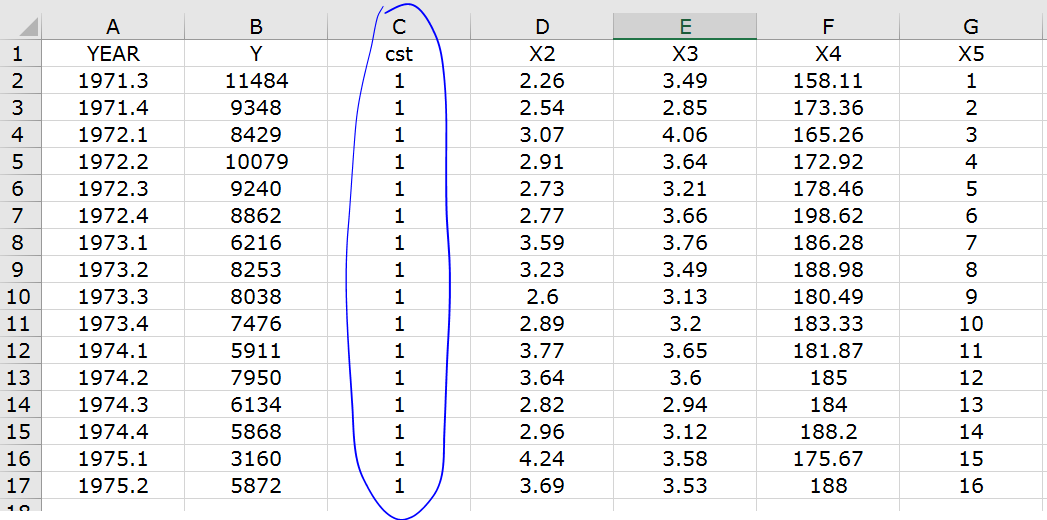
\includegraphics[width=14.54in,height=8in]{picture/lab4-matrix/handle-data} 

   }

   \caption{Excel数据与变量预处理}\label{fig:handle-data}
   \end{figure}
\item
  构造组(group)对象xg

  \begin{itemize}
  \tightlist
  \item
    提示:把因变量\texttt{X}序列(series)和常数\texttt{cst}序列(series)对象一起转换成矩阵(matrix)对象
  \item
    得到序列组\(X\)

    \begin{itemize}
    \tightlist
    \item
      命名:建议将样本数据序列组的Eviews对象命名为xg
    \item
      菜单:依次选择(
      \texttt{cst\ ln\_x2\ ln\_x3\ ln\_x4\ x5})---\textgreater{}open as
      group ---\textgreater{}name(建议命名为xg)
    \end{itemize}
  \end{itemize}
\item
  得到矩阵\(\mathbf{X}\)

  \begin{itemize}
  \tightlist
  \item
    命名:建议将样本数据矩阵\(\mathbf{X}\)的Eviews对象命名为x
  \item
    命令:matrix x=xg
  \end{itemize}
\end{itemize}

\hypertarget{mathbfhatbetasrm_2}{%
\subsection{\texorpdfstring{计算直线回归方程的回归系数向量(\(\mathbf{\hat{\beta}}\)),并写出样本回归模型(\(SRM_2\))。}{计算直线回归方程的回归系数向量(\textbackslash{}mathbf\{\textbackslash{}hat\{\textbackslash{}beta\}\}),并写出样本回归模型(SRM\_2)。}}\label{mathbfhatbetasrm_2}}

\begin{itemize}
\item
  目标:根据理论的矩阵公式,计算得到直线回归方程的回归系数向量(\(\mathbf{\hat{\beta}}\))
\item
  思路:
\item
  构造矩阵\(\mathbf{y}\)

  \begin{itemize}
  \tightlist
  \item
    提示:把因变量\texttt{Y}序列(series)对象转化成矩阵对象
  \item
    命名:建议将样本数据矩阵\(\mathbf{y}\)的Eviews对象命名为y
    +命令:matrix y=q
  \end{itemize}
\item
  构造矩阵\(\mathbf{X}\)

  \begin{itemize}
  \tightlist
  \item
    提示:把因变量\texttt{X}序列(series)对象转化成矩阵对象
  \item
    得到序列组\(X\)

    \begin{enumerate}
    \def\labelenumi{\alph{enumi}.}
    \tightlist
    \item
      命名:建议将样本数据序列组\(X\)的Eviews对象命名为xg
    \item
      菜单:依次选择(
      \texttt{cst\ ln\_x2\ ln\_x3\ ln\_x4\ x5})---\textgreater{}open as
      group ---\textgreater{}name(建议命名为xg)
    \end{enumerate}
  \item
    得到矩阵\(\mathbf{X}\):

    \begin{enumerate}
    \def\labelenumi{\alph{enumi}.}
    \tightlist
    \item
      命名:建议将样本数据矩阵\(\mathbf{X}\)的Eviews对象命名为x
    \item
      命令:matrix x=xg
    \end{enumerate}
  \end{itemize}
\item
  利用矩阵公式计算回归系数(\(\mathbf{\hat{\beta}}\))

  \begin{itemize}
  \tightlist
  \item
    得到重要矩阵\(\mathbf{(X'X)}\)

    \begin{enumerate}
    \def\labelenumi{\alph{enumi}.}
    \tightlist
    \item
      命名:建议将重要矩阵\(\mathbf{(X'X)}\)的Eviews对象命名为xtx
    \item
      命令:matrix
      \href{mailto:xtx=@transpose}{\nolinkurl{xtx=@transpose}}(x)*x
    \end{enumerate}
  \item
    得到重要矩阵\(\mathbf{{(X'X)}^{-1}}\)

    \begin{enumerate}
    \def\labelenumi{\alph{enumi}.}
    \tightlist
    \item
      命名:建议将重要矩阵\(\mathbf{{(X'X)}^{-1}}\)的Eviews对象命名为xtxi
    \item
      命令: matrix
      \href{mailto:xtxi=@inverse}{\nolinkurl{xtxi=@inverse}}(xtx)
    \end{enumerate}
  \item
    得到重要矩阵\(\mathbf{X'y}\)(建议命名为xty)

    \begin{enumerate}
    \def\labelenumi{\alph{enumi}.}
    \item
      命名:建议将重要矩阵\(\mathbf{X'y}\)的Eviews对象命名为xty
    \item
      命令: matrix
      \href{mailto:xty=@transpose}{\nolinkurl{xty=@transpose}}(x)*y
    \end{enumerate}
  \item
    得到回归系数矩阵\(\mathbf{\hat{\beta}}\)

    \begin{enumerate}
    \def\labelenumi{\alph{enumi}.}
    \item
      提示:回归系数矩阵\(\mathbf{\hat{\beta}}\)的理论计算公式为
      \[\mathbf{\hat{\beta}}=\mathbf{{(X'X)}^{-1}X'y}\]
    \item
      命名:建议将回归系数矩阵\(\mathbf{\hat{\beta}}\)的Eviews对象命名为beta\_hat
    \item
      命令:matrix beta\_hat=xtxi*xty
    \end{enumerate}
  \end{itemize}
\end{itemize}

\hypertarget{hatsigma2hatsigma}{%
\subsection{\texorpdfstring{计算回归误差方差(\(\hat{\sigma}^2\))和回归误差标准差(\(\hat{\sigma}\))}{计算回归误差方差(\textbackslash{}hat\{\textbackslash{}sigma\}\^{}2)和回归误差标准差(\textbackslash{}hat\{\textbackslash{}sigma\})}}\label{hatsigma2hatsigma}}

\begin{itemize}
\tightlist
\item
  目标:根据理论的矩阵公式,回归误差方差(\(\hat{\sigma}^2\))和回归误差标准差(\(\hat{\sigma}\))
\item
  思路:
\item
  提示:回归误差方差(\(\hat{\sigma}^2\))和回归误差标准差(\(\hat{\sigma}\))的理论计算公式分别为:
\end{itemize}

\[\hat{\sigma}^2=\frac{\sum{e_i^2}}{n-k}=\frac{\mathbf{y'y-\hat{\beta}'X'y}}{n-k}\]
\[\hat{\sigma}=\sqrt{\frac{\sum{e_i^2}}{n-k}}=\sqrt{\frac{\mathbf{yy'-\hat{\beta}'X'y}}{n-k}}\]

\begin{itemize}
\item
  命名:建议将回归误差方差的Eviews对象命名为sigma2\_hat,将回归误差标准差的Eviews对象命名为sigma\_hat。
\item
  命令:

  \begin{itemize}
  \tightlist
  \item
    回归误差方差\(\hat{\sigma}^2\): scalar
    sigma2\_hat=1/(16-5)\emph{(@transpose(y)}\href{mailto:y-@transpose}{\nolinkurl{y-@transpose}}(beta\_hat)*xty)
  \item
    回归误差标准差 \(\hat{\sigma}\):
    \href{mailto:scalarsigma_hat=@sqr}{\nolinkurl{scalarsigma\_hat=@sqr}}(sigma2\_hat)
  \end{itemize}
\item
  注意:与eviews报告比对是否正确(注:要开根号才能比较!)
\end{itemize}

\hypertarget{widehatvar_widehatcovmathbfhatbeta}{%
\subsection{\texorpdfstring{计算回归系数的样本方差协方差矩阵(\(\widehat{var}\_\widehat{cov}(\mathbf{\hat{\beta}})\))}{计算回归系数的样本方差协方差矩阵(\textbackslash{}widehat\{var\}\textbackslash{}\_\textbackslash{}widehat\{cov\}(\textbackslash{}mathbf\{\textbackslash{}hat\{\textbackslash{}beta\}\}))}}\label{widehatvar_widehatcovmathbfhatbeta}}

\begin{itemize}
\tightlist
\item
  目标:根据理论的矩阵公式,计算回归系数的样本方差协方差矩阵(\(\widehat{var}\_\widehat{cov}(\mathbf{\hat{\beta}})\))
\item
  思路:
\item
  提示:回归系数的样本方差协方差矩阵阵(\(\widehat{var}\_\widehat{cov}(\mathbf{\hat{\beta}})\))的理论计算公式为:
\end{itemize}

\[\widehat{var}\_\widehat{cov}(\mathbf{\hat{\beta}})=\hat{\sigma}^2\mathbf{(X'X)^{-1}}\]

\begin{itemize}
\tightlist
\item
  命名:建议将样本方差协方差矩阵的Eviews对象命名为s2\_varcov\_beta\_hat
\item
  命令:matrix s2\_varcov\_beta\_hat=sigma2\_hat*xtxi
\item
  注意:与eviews报告比对是否正确(注:要开根号才能比较!)
\end{itemize}

\subsection{得出回归系数的样本标准差向量()}

\begin{itemize}
\item
  目标:根据理论的矩阵公式,得出回归系数的样本标准差向量()
\item
  思路:
\item
  提取矩阵主对角元素,得到方差向量\(\mathbf{S_{\hat{\beta}}^2}\)

  \begin{itemize}
  \tightlist
  \item
    提示:该矩阵维度为5*5
  \item
    命名:建议将方差向量的Eviews对象命名为s2\_beta\_hat
  \item
    命令:matrix
    \href{mailto:s2_beta_hat=@getmaindiagonal}{\nolinkurl{s2\_beta\_hat=@getmaindiagonal}}(s2\_varcov\_beta\_hat)
  \item
    注意:Eviews命令\texttt{@getmaindiagonal()}的作用是提取矩阵的对角线元素
  \end{itemize}
\item
  矩阵元素开根号,得到标准差向量

  \begin{itemize}
  \tightlist
  \item
    提示:标准差向量的矩阵维度为5*1
  \item
    命名:建议将标准差向量的Eviews对象命名为
  \item
    命令:matrix =@sqr(s2\_beta\_hat)
  \item
    注意:与eviews报告比对是否正确
  \end{itemize}
\end{itemize}

\hypertarget{tssessrss}{%
\subsection{\texorpdfstring{进行平方和分解,计算\(TSS\)、\(ESS\)和\(RSS\)}{进行平方和分解,计算TSS、ESS和RSS}}\label{tssessrss}}

\begin{itemize}
\tightlist
\item
  目标:根据理论的矩阵公式,进行平方和分解,计算\(TSS\)、\(ESS\)和\(RSS\)
\item
  思路:
\item
  计算均值修正值\(n\bar{Y}^2\)

  \begin{itemize}
  \tightlist
  \item
    提示:均值修正值的理论公式为
  \end{itemize}

  \[n\bar{Y}^2\]

  \begin{itemize}
  \item
    命名:建议将均值修正值的Eviews对象命名为mean\_adj
  \item
    命令:scalar mean\_adj=16*(@mean(y))\^{}2
  \end{itemize}
\item
  计算总平方和\(TSS\)

  \begin{itemize}
  \tightlist
  \item
    提示:总平方和\(TSS\)的理论计算公式为
  \end{itemize}

  \[TSS=\mathbf{y'y}-n\bar{Y}^2\]

  \begin{itemize}
  \item
    命名:建议将总平方和的Eviews对象命名为tss
  \item
    命令:scalar
    \href{mailto:tss=@transpose}{\nolinkurl{tss=@transpose}}(y)*y-mean\_adj
  \end{itemize}
\item
  计算残差平方和\(RSS\)

  \begin{itemize}
  \tightlist
  \item
    提示:残差平方和\(RSS\)的理论计算公式为:
  \end{itemize}

  \[RSS=\mathbf{e'e}=\mathbf{y'y-\hat{\beta}'X'y}\]

  \begin{itemize}
  \item
    命名:建议将残差平方和的Eviews对象命名为rss
  \item
    命令:scalar
    \href{mailto:rss=@transpose}{\nolinkurl{rss=@transpose}}(y)\emph{\href{mailto:y-@transpose}{\nolinkurl{y-@transpose}}(beta\_hat)}xty
  \item
    注意:与eviews报告比对是否正确
  \end{itemize}
\item
  计算回归平方和\(ESS\)

  \begin{itemize}
  \tightlist
  \item
    提示:回归平方和\(ESS\)的理论计算公式为:
  \end{itemize}

  \[ESS=\mathbf{e'e}=\mathbf{\hat{\beta}'X'y}-n\bar{Y}^2\]

  \begin{itemize}
  \item
    命名:建议将回归平方和的Eviews对象命名为ess
  \item
    命令:scalar
    \href{mailto:ess=@transpose}{\nolinkurl{ess=@transpose}}(beta\_hat)*xty-mean\_adj
  \end{itemize}
\end{itemize}

\hypertarget{r2barr2}{%
\subsection{\texorpdfstring{计算判定系数\(R^2\)和调整判定系数(\(\bar{R}^2\))}{计算判定系数R\^{}2和调整判定系数(\textbackslash{}bar\{R\}\^{}2)}}\label{r2barr2}}

\begin{itemize}
\tightlist
\item
  目标:根据理论的矩阵公式,计算判定系数\(R^2\)和调整判定系数(\(\bar{R}^2\))
\item
  思路:
\item
  计算判定系数\(R^2\)

  \begin{itemize}
  \tightlist
  \item
    提示:理论计算公式为:
  \end{itemize}

  \[R^2=\frac{ESS}{TSS}=\frac{\mathbf{\hat{\beta}'X'y}-n\bar{Y}^2}{\mathbf{y'y}-n\bar{Y}^2}\]

  \begin{itemize}
  \tightlist
  \item
    命名:建议将判定系数的Eviews对象命名为r2
  \item
    命令:scalar r2=ess/tss
  \item
    注意:与eviews报告比对是否正确
  \end{itemize}
\item
  计算调整判定系数(\(\bar{R}^2\))

  \begin{itemize}
  \tightlist
  \item
    提示:判定系数\(\bar{R}^2\)的理论计算公式为
  \end{itemize}

  \[\bar{R}^2=1-\frac{RSS/{f_{RSS}}}{TSS/{f_{TSS}}}=1-\frac{\mathbf{y'y-\hat{\beta}X'y}/{n-k}}{{(\mathbf{y'y}-n\bar{Y}^2)}/{n-1}}\]

  \begin{itemize}
  \tightlist
  \item
    命名:建议将调整判定系数的Eviews对象命名为r2\_adj
  \item
    命令:scalar r2\_adj=1-(rss/11)/(tss/15)
  \item
    注意:与eviews报告比对是否正确
  \end{itemize}
\end{itemize}

\hypertarget{tmathbftast_beta}{%
\subsection{\texorpdfstring{计算得到样本t统计量(\(\mathbf{t^{\ast}_{\beta}}\))}{计算得到样本t统计量(\textbackslash{}mathbf\{t\^{}\{\textbackslash{}ast\}\_\{\textbackslash{}beta\}\})}}\label{tmathbftast_beta}}

\begin{itemize}
\tightlist
\item
  目标:根据理论的矩阵公式,计算样本t统计量(\(\mathbf{t^{\ast}_{\beta}}\)),并进行t假设检验
\item
  思路:
\item
  提示:样本t统计量\(\mathbf{t^{\ast}_{\beta}}\)的理论计算公式为
\end{itemize}

\[\mathbf{t^{\ast}_{\beta}=\frac{\hat{\beta}}{S_{\hat{\beta}}}}\]

\begin{itemize}
\tightlist
\item
  命名:建议将样本t统计量的Eviews对象命名为t\_str\_beta\_hat\\
\item
  命令:matrix
  \href{mailto:t_str_beta_hat=@ediv}{\nolinkurl{t\_str\_beta\_hat=@ediv}}(beta\_hat,s\_beta\_hat)
\item
  注意:与Eviews报告比对是否正确。Eviews命令\texttt{@ediv()}的作用是将矩阵对应元素进行相除。
\end{itemize}

\hypertarget{alpha0.05tt_1-alpha2n-kt}{%
\subsection{\texorpdfstring{计算给定\(\alpha=0.05\)水平下的查表的理论t值(\(t_{1-\alpha/2}(n-k)\)),并进行t假设检验}{计算给定\textbackslash{}alpha=0.05水平下的查表的理论t值(t\_\{1-\textbackslash{}alpha/2\}(n-k)),并进行t假设检验}}\label{alpha0.05tt_1-alpha2n-kt}}

\begin{itemize}
\tightlist
\item
  目标:根据理论的矩阵公式,计算查表的理论t值(\(t_{1-\alpha/2}(n-k)\)),并进行t假设检验
\item
  思路:
\item
  提示:查表的理论t值(\(t_{1-\alpha/2}(n-k)\))的理论计算公式为:
\end{itemize}

\[t_{1-\alpha/2}(n-k)=t_{0.975}(11)\]

\begin{itemize}
\tightlist
\item
  命名:建议将查表理论t值的Eviews对象命名为t\_value
\item
  命令:scalar
  \href{mailto:t_value=@qtdist}{\nolinkurl{t\_value=@qtdist}}(0.975,11)
\end{itemize}

\hypertarget{f}{%
\subsection{对回归方程的整体显著性进行F假设检验}\label{f}}

\begin{itemize}
\tightlist
\item
  目标:根据理论的矩阵公式,计算样本F统计量,并进行模型整体显著性检验
\item
  思路:
\item
  提示:样本F统计量\(F^{\ast}\)的理论计算公式为:
\end{itemize}

\[F^{\ast}=\frac{ESS/{f_{ESS}}}{RSS/{f_{RSS}}}=\frac{MSS_{ESS}}{MSS_{RSS}}=\frac{(\mathbf{\hat{\beta}X'y}-n\bar{Y}^2)/{k-1}}{{(\mathbf{y'y-\hat{\beta}'X'y})}/{n-k}}\]

\begin{itemize}
\tightlist
\item
  命名:建议将样本F统计量的Eviews对象命名为f\_str\\
\item
  命令:scalar f\_str=(ess/4)/(rss/11)
\item
  注意:与eviews报告比对是否正确。
\end{itemize}

\hypertarget{alpha0.05ff_1-alphak-1n-kf}{%
\subsection{\texorpdfstring{计算给定\(\alpha=0.05\)水平下的查表的理论F值(\(F_{1-\alpha}(k-1,n-k)\)),并进行F假设检验}{计算给定\textbackslash{}alpha=0.05水平下的查表的理论F值(F\_\{1-\textbackslash{}alpha\}(k-1,n-k)),并进行F假设检验}}\label{alpha0.05ff_1-alphak-1n-kf}}

\begin{itemize}
\tightlist
\item
  目标:根据理论的矩阵公式,计算查表的理论F值(\(F_{1-\alpha}(k-1,n-k)\)),并进行F假设检验
\item
  思路:
\item
  提示:查表的理论F值(\(F_{1-\alpha}(k-1,n-k)\))的理论计算公式为:
\end{itemize}

\[F_{1-\alpha}(k-1,n-k)=F_{0.95}(4,11)\]

\begin{itemize}
\tightlist
\item
  命名:建议将查表理论F值的Eviews对象命名为f\_value
\item
  命令:scalar
  \href{mailto:t_value=@qfdist}{\nolinkurl{t\_value=@qfdist}}(0.95,4,11)
\end{itemize}

\hypertarget{eyxx_0}{%
\subsection{\texorpdfstring{对回归方程的进行样本外均值预测\(E(Y|X=X_0)\)}{对回归方程的进行样本外均值预测E(Y\textbar{}X=X\_0)}}\label{eyxx_0}}

\begin{itemize}
\item
  目标:根据理论的矩阵公式,计算样本外的均值预测(\(E(Y|X=X_0)\))
\item
  思路:
\item
  构造\(X_0\)矩阵

  \begin{itemize}
  \tightlist
  \item
    提示:已知给定的样本外数据为\((X_{20}=20,X_{30}=4,X_{40}=4,X_{50}=200)\)。此时,\(X_0\)矩阵的理论构造表达式为:
  \end{itemize}

  \[\mathbf{X_0}= \begin{bmatrix}1 & X_{20} & X_{30} & X_{40} & X_{50}\\\end{bmatrix}\]

  \begin{itemize}
  \tightlist
  \item
    命名:建议将样本外预测矩阵\(X_0\)的Eviews对象命名为x0
  \item
    命令:

    \begin{enumerate}
    \def\labelenumi{\alph{enumi}.}
    \tightlist
    \item
      产生空矩阵:matrix(1,5) x0
    \item
      给矩阵赋值:matrix.fill(b=r) 1,20,4,4,200
    \end{enumerate}
  \item
    注意:与eviews报告比对是否正确。
  \end{itemize}
\item
  计算样本外预测值(\(\hat{Y}_0\))

  \begin{itemize}
  \tightlist
  \item
    提示:样本外预测值(\(\hat{Y}_0\))的计算公式为:
  \end{itemize}

  \[\mathbf{\hat{Y_0}=X_0\hat{\beta}}\]

  \begin{itemize}
  \item
    命名:建议将样本外预测值\(\hat{Y}_0\)的Eviews对象命名为forecast\_exp
  \item
    命令:matrix Y0\_hat=x0*beta\_hat
  \item
    注意:与eviews报告比对是否正确。
  \end{itemize}
\item
  计算样本外预测值(\(\hat{Y}_0\))的样本标准差\(S_{\hat{Y}_0}\)

  \begin{itemize}
  \tightlist
  \item
    提示:样本外预测值\(\hat{Y}_0\)的样本标准差\(S_{\hat{Y}_0}\)的理论计算公式为:
  \end{itemize}

  \[\mathbf{S_{\hat{Y_0}}= \sqrt{\hat{\sigma}^2X_0(X'X)^{-1}X_0'}}\]

  \begin{itemize}
  \item
    命名:建议将样本标准差\(S_{\hat{Y}_0}\)的Eviews对象命名为s\_y0h
  \item
    命令:scalar
    \href{mailto:s_y0h=@sqr}{\nolinkurl{s\_y0h=@sqr}}(\href{mailto:sigma2_hat*x0*xtxi*@transpose}{\nolinkurl{sigma2\_hat*x0*xtxi*@transpose}}(x0))
  \item
    注意:与eviews报告比对是否正确。
  \end{itemize}
\item
  计算均值预测的\(E(Y|X=X_0)\)置信区间

  \begin{itemize}
  \tightlist
  \item
    提示:均值预测的\(E(Y|X=X_0)\)置信区间的理论计算公式为:
  \end{itemize}

  \[\mathbf{\hat{Y_0}-t_{1-\alpha/2}(n-k)\cdot S_{\hat{Y_0}}\leq {E(Y|X=X_0)}\leq \hat{Y_0}+t_{1-\alpha/2}(n-k)\cdot S_{\hat{Y_0}}}\]

  \begin{itemize}
  \tightlist
  \item
    命名:建议将均值预测\(E(Y|X=X_0)\)置信区间左界的Eviews对象命名为y\_exp\_lft;右界的Eviews对象命名为y\_exp\_rht
  \item
    命令:

    \begin{enumerate}
    \def\labelenumi{\alph{enumi}.}
    \tightlist
    \item
      左界:scalar y\_exp\_lft=Y0\_hat-t\_value*s\_y0h
    \item
      右界:scalar y\_exp\_rht=Y0\_hat+t\_value*s\_y0h
    \end{enumerate}
  \item
    注意:与eviews报告比对是否正确。
  \end{itemize}
\end{itemize}

\hypertarget{y_0xx_0}{%
\subsection{\texorpdfstring{对回归方程的进行样本外个值预测\((Y_0|X=X_0)\)}{对回归方程的进行样本外个值预测(Y\_0\textbar{}X=X\_0)}}\label{y_0xx_0}}

\begin{itemize}
\tightlist
\item
  计算随机变量\({(\hat{Y}_0-Y_0)}\)的样本标准差\(S_{(\hat{Y}_0-Y_0)}\)

  \begin{itemize}
  \tightlist
  \item
    提示:随机变量\({(\hat{Y}_0-Y_0)}\)的样本标准\(S_{(\hat{Y}_0-Y_0)}\)的理论计算公式为:
  \end{itemize}

  \[\mathbf{S_{(\hat{Y}_0-Y_0)}=\sqrt{\hat{\sigma}^2(1+X_0(X'X)^{-1}X_0')}}\]

  \begin{itemize}
  \item
    命名:建议将随机变量\({(\hat{Y}_0-Y_0)}\)的样本标准差\(S_{(\hat{Y}_0-Y_0)}\)的Eviews对象命名为s\_y0h\_mns\_y0
  \item
    命令:scalar
    \href{mailto:s_y0h_mns_y0=@sqr}{\nolinkurl{s\_y0h\_mns\_y0=@sqr}}(sigma2\_hat*(\href{mailto:1+x0*xtxi*@transpose}{\nolinkurl{1+x0*xtxi*@transpose}}(x0)))
  \item
    注意:与eviews报告比对是否正确。
  \end{itemize}
\item
  计算个值预测的\((Y_0|X=X_0)\)置信区间

  \begin{itemize}
  \tightlist
  \item
    提示:均值预测的\((Y_0|X=X_0)\)置信区间的理论计算公式为:
  \end{itemize}

  \[\mathbf{\hat{Y_0}-t_{1-\alpha/2}(n-k)\cdot S_{(\hat{Y_0}-Y_0)}\leq{(Y_0|X=X_0)}\leq \hat{Y_0}+t_{1-\alpha/2}(n-k)\cdot S_{(\hat{Y_0}-Y_0)}} \]

  \begin{itemize}
  \item
    命名:建议将均值预测\((Y_0|X=X_0)\)置信区间左界的Eviews对象命名为y\_ind\_lft;右界的Eviews对象命名为y\_ind\_rht
  \item
    命令:

    \begin{enumerate}
    \def\labelenumi{\alph{enumi}.}
    \tightlist
    \item
      左界:scalar y\_ind\_lft=Y0\_hat-t\_value*s\_y0h\_mns\_y0
    \item
      右界:scalar y\_ind\_rht=Y0\_hat+t\_value*s\_y0h\_mns\_y0
    \end{enumerate}
  \item
    注意:与eviews报告比对是否正确。
  \end{itemize}
\end{itemize}


\end{document}
